\chapter{Applications of Cryptographic Hash Functions}
\label{chap:hash_applications}

This chapter is devoted to applications of \glsfirstplural{hash function}.



\section{Ethereum Addresses}

This section assumes some knowledge of the \gls{ethereum} blockchain and
\glspl{elliptic curve}.

\subsection{Address Definition}

We recall that \gls{ethereum} uses \textsc{secp256k1}
for its \gls{ecc};
its private keys are 256-bit nonnegative (unsigned) integers
(32 bytes in length; 64 hexadecimal characters).
Each private key $k$ produces a public key

\begin{equation}
    P = k\cdot G;
\end{equation}

\noindent
here, $G$ is the specified base point of the \gls{elliptic curve}.
Uncompressed, the public key is two 256-bit unsigned integers
(64 bytes).
With the compressed or uncompressed designation byte,
a public key is either 65 bytes uncompressed or 33 bytes compressed.

This is a significant amount of space.
In order to save space, \gls{ethereum}~\cite[Eq.~314]{EthereumYellowpaper}
defines the address of every public key.
This is computed by performing the \Keccak{} hash of the public key
and using the rightmost 20 bytes.

\subsection{Colliding Addresses}

While each private key corresponds to a unique public key,
using only 20 bytes of a hash output reduces the unique
number of addresses to $2^{160}$.
Because there are approximately $2^{256}$ unique private and public keys,
this means there are \emph{many} public keys with the same address;
a rough estimate would be that there are approximately $2^{96}$ public keys
per address.

The good news is that, due to \Keccak{} being a strong \gls{hash function}
with collision resistance,
finding any 2 public keys which map to the same address would require
the computation of approximately $2^{80}$ hash values.
Although large, it \emph{may} be possible for this many hash operations
to be computed by a \emph{well-funded and dedicated} adversary.

In practice, an adversary would want to find a private key
corresponding to a \emph{particular} address.
This converts a collision attack into a second-preimage attack.
This instead requires approximately $2^{160}$ hash operations
to find a valid public key.
Considering the belief that performing $2^{128}$ operations is impractical,
performing $2^{160}$ is also impractical.
Thus, there is little concern for colliding addresses in \gls{ethereum}
even though they certainly exist.

\subsection{Example}

\begin{example}[Ethereum Address]
\exampleCodeReference{examples/hash\_applications/ethereum\_addr.py}

We have the private key

\begin{align}
    k &= 2^{248} + 1 \nonumber\\
&= \texttt{0100000000000000000000000000000000000000000000000000000000000001};
\end{align}

\noindent
the second line lists the private key in hexadecimal form.
The corresponding public key in hexadecimal form is

\begin{align}
    &P = k\cdot G = \nonumber\\
    &(\texttt{e4dbb4350d84eabec1d67e40a398a78a8e6d719d86914393fca83b88dbe927af},
        \nonumber\\
    &\texttt{b80fe66bf659859889a544623c945d0bd80d855f649e8c197be3aa41fe0390f8}).
\end{align}

\noindent
By computing the \Keccak{}-256 hash of this and taking the rightmost
20 bytes, we see

\begin{equation}
    \texttt{addr} = \texttt{7691ee0343b9a529675e1a8a70197b3b704f90b7}.
\end{equation}

\noindent
This address is much more manageable than the public key.
\end{example}



\section{Commitment Schemes}

A \emph{commitment scheme} is a method to commit to a specific value
without revealing any information about the value;
at a later point in time, it is possible to reveal the committed
value and prove that this particular value was the commitment.
Ideally, a commitment scheme is \emph{hiding} and \emph{binding}:
\emph{hiding} because no information about the committed value is revealed;
\emph{binding} because the committed value cannot be changed after
it is committed.

Suppose we have our \gls{hash function} $H:\braces{0,1}^{*}\to\braces{0,1}^{n}$.
If $m\in\braces{0,1}^{*}$ is the value to be committed,
we choose our random value $r\chooseRandom{}\braces{0,1}^{n}$.
The commitment is then

\begin{equation}
    c \mathDef{} H(r||m).
\end{equation}

\noindent
At a future point in time, revealing the value $m$ and the random value $r$
will show that $m$ was the value previously committed.
This is due to the fact that it is difficult to determine
$r'\in\braces{0,1}^{n}$ and $m'\in\braces{0,1}^{*}$
such that $c = H(r'||m')$.

\begin{example}[Commitment Scheme]
\exampleCodeReference{examples/hash\_applications/commitment\_scheme.py}

We look at a commitment scheme using \MDFive{};
see Listing~\ref{list:commitment_scheme_md5}.
We are seeking to commit to the byte value

\begin{equation}
    m \mathDef{} \texttt{01}.
\end{equation}

\noindent
The random value $r$ is the \MDFive{} hash of 16 zero bytes:

\begin{equation}
    r \mathDef{} \texttt{4ae71336e44bf9bf79d2752e234818a5}.
\end{equation}

\noindent
The resulting commitment $c$ is then

\begin{align}
    c &\mathDef{} \text{\MDFive{}}\parens{r||m} \nonumber\\
        &= \texttt{ff95213ae708e6443c5f0ae2d8f5fe41}.
\end{align}

\noindent
At a later point in time, $m$ and $r$ may be revealed.

\lstset{
    showstringspaces=false,
    frame=single
}
\lstinputlisting[
    label=list:commitment_scheme_md5,
    float,
    language=Python,
    caption={Commitment scheme using \MDFive{}}]{code/hash_applications/commitment_scheme.py}


\emph{Note well:} We note that in an actual commitment scheme,
such a random value \emph{should not be used};
the value should be truly random or drawn from a \glsfirst{csprng}.
\end{example}

It is not necessary that $r$ be a bit string of length $n$
in the commitment scheme;
this was chosen for convenience.
Even so, it must be long enough so that it is impractical
to test every possible value for $r$ and $m$.
If the random value $r$ was not included in the commitment,
problems may arise.
If the commitment was just $H(m)$,
it may be possible to compute all possible values
and determine which value is committed;
thus, the scheme would not be hiding.



\section{Hash Chains}

Hash chains use \glspl{hash function} recursively.
If $H$ is a \gls{hash function}, then a hash chain of $x$ is

\begin{equation}
    x, H(x), H(H(x)), H(H(H(x))), H(H(H(H(x)))), \cdots
\end{equation}

\noindent
This can be more compactly written as

\begin{equation}
    H^{0}(x), H^{1}(x), H^{2}(x), H^{3}(x), H^{4}(x), \cdots
\end{equation}

\noindent
where we have

\begin{equation}
    H^{n}(x) = \begin{cases}
            x\quad &n = 0 \\
            H(H^{n-1}(x))\quad &n \ge 1 \\
    \end{cases}.
\end{equation}

\noindent
Depending on the circumstance, the initial value ($x$ or $H^{0}(x)$)
may not be included.

Hash chains enable easy iteration in the forward direction.
By using a secure \gls{hash function}, it is impractical to iterate in reverse,
as doing so would require computing \gls{hash function} preimages.

\begin{example}[Hash Chain]
\exampleCodeReference{examples/hash\_applications/hash\_chain.py}

We look at a hash chain using \MDFive{};
see Listing~\ref{list:hash_chain_md5}.
The initial byte array is

\begin{align}
    x &= H^{0}(x) \nonumber\\
        &= \texttt{00112233445566778899aabbccddeeff}.
\end{align}

\lstset{
    showstringspaces=false,
    frame=single
}
\lstinputlisting[
    label=list:hash_chain_md5,
    float,
    language=Python,
    caption={Hash chain using \MDFive{}}]{code/hash_applications/hash_chain.py}


\noindent
Iterating \MDFive{} five times gives us the value

\begin{equation}
    H^{5}(x) = \texttt{e94712ae81bf26d81b0e7475fbf6b3f8}.
\end{equation}
\end{example}



\section{Merkle Trees}

Another useful application of \glspl{hash function} are \emph{Merkle Trees}.

\subsection{Intuition}

It is challenging to send large amounts of data at one time.
It would be convenient to chop the data into small pieces
and then send those small pieces of data separately.
The challenge is then to ensure the validity of each small
piece of data.

A \emph{Merkle Tree} can help solve this problem.
It uses one cryptographic hash value to represent the \emph{entire}
collection of data.
At the same time, individual blocks of data can be retrieved
along with its associated \emph{Merkle Proof}:
a proof which shows the individual data block is valid.

\subsection{Definition}

The algorithm defining the Merkle Tree root hash can be found in
Alg.~\ref{alg:merkle_tree};
see Alg.~\ref{alg:merkle_proof} for the proof of inclusion.
These definitions are modified
from~\cite[Chapter 8.9]{BonehShoupGraduateApplied}.

\begin{algorithm}[p]
\caption{Compute Merkle Tree root hash}
\label{alg:merkle_tree}
\begin{algorithmic}[1]
\Require $n = 2^{k}$ for some $k\ge1$; $H$ is a \gls{hash function}.
\Procedure{MerkleTreeRoot}{$x_{0}, x_{1}, \cdots, x_{n-1}$}
    \For {$i=0; i < n; i{+}{+}$}
        \State $y_{i} \algAssign{} H(x_{i})$
        \Comment{Compute leaf hashes}
    \EndFor
    \For {$i=0; i < n-1; i{+}{+}$}
        \State $y_{n+i} \algAssign{} H(y_{2i}\|y_{2i+1})$
        \Comment{Compute internal hashes}
    \EndFor
    \State \Return $y_{2n-2}$
    \Comment{Return root hash}
\EndProcedure
\end{algorithmic}
\end{algorithm}

\begin{algorithm}[p]
\caption{Validate Merkle Proof of Inclusion}
\label{alg:merkle_proof}
\begin{algorithmic}[1]
\Require $n = 2^{k}$ for some $k\ge1$; $H$ is a \gls{hash function}; $\text{len}(\pi) = \log_{2}(n)$.
\Procedure{ValidateMerkleProof}{$x, i, y_{2n-2}, \pi$}
    \State $\hat{y}_{i} \algAssign{} H(x)$
    \Comment{Compute leaf hash}
    \State $\mu \algAssign{} i$
    \For {$k=0; k < \log_{2}(n); k{+}{+}$}
        \If {$\mu$ odd}
            \State $\ell \algAssign{} (\mu-1)/2$
            \State $\nu \algAssign{} n + \ell$
            \State $\hat{y}_{\nu} \algAssign{} H(\pi_{k}\|\hat{y}_{\mu})$
        \Else
            \State $\ell \algAssign{} \mu/2$
            \State $\nu \algAssign{} n + \ell$
            \State $\hat{y}_{\nu} \algAssign{} H(\hat{y}_{\mu}\|\pi_{k})$
        \EndIf
        \State $\mu \algAssign{} \nu$
    \EndFor
    \If {$\hat{y}_{2n-2} = y_{2n-2}$}
        \State \Return \texttt{true}
    \Else
        \State \Return \texttt{false}
    \EndIf
\EndProcedure
\end{algorithmic}
\end{algorithm}


\subsection{Continued Discussion}

As mentioned above, there is an associated proof of inclusion
for each piece of data.
These individual proofs are inexpensive.
It is possible to perform multiple inclusion-proofs at once;
this is a called a \emph{Merkle Multi-Proof}.
We will not give a formal definition of a multi-proof
but see Example~\ref{example:hash_app_merkle_tree_multi-proof}
for an example.

We note the following details which are useful
but which will not be discussed any further here.
In addition to proofs of inclusion,
it is also possible to have \emph{proofs of exclusion};
doing this requires additional assumptions on the
input data~\cite{EfficientSMT}.
Furthermore, some implementations may use prefixes when hashing;
the purpose of this is to provide
second-preimage resistance~\cite{rfc6962,rfc9162}.

\subsection{Examples}

\begin{example}[2-Layer Merkle Tree]
\exampleCodeReference{examples/hash\_applications/merkle\_tree\_md5\_2.py}

We begin by starting with an example involving 4 blocks of data;
see the Merkle Tree in Figure~\ref{fig:merkle_tree_2}
for the example.

\begin{figure}[p]
\centering
\begin{subfigure}{\textwidth}
    \centering
    \begin{tikzpicture}
        [level 1/.style={sibling distance=40mm},
         level 2/.style={sibling distance=20mm}]
        \node[circle,draw] (root) {$H$}
            child {node[circle,draw] {$H$}
                child {node[circle,draw] {$H$}
                    child {node[rectangle,draw] {$x_{1}$}
                    edge from parent[<-,thick]}
                edge from parent[<-,thick]
                    node[left] {$y_{1}$}
                }
                child {node[circle,draw] {$H$}
                    child {node[rectangle,draw] {$x_{2}$}
                    edge from parent[<-,thick]}
                edge from parent[<-,thick]
                    node[right] {$y_{2}$}
                }
            edge from parent[<-,thick]
                node[left] {$y_{5}$}
            }
            child {node[circle,draw] {$H$}
                child {node[circle,draw] {$H$}
                    child {node[rectangle,draw] {$x_{3}$}
                    edge from parent[<-,thick]}
                edge from parent[<-,thick]
                    node[left] {$y_{3}$}
                }
                child {node[circle,draw] {$H$}
                    child {node[rectangle,draw] {$x_{4}$}
                    edge from parent[<-,thick]}
                edge from parent[<-,thick]
                    node[right] {$y_{4}$}
                }
            edge from parent[<-,thick]
                node[right] {$y_{6}$}
            };
        \node[above=of root] (header) {};
        \draw[->,thick] (root) to node[auto,swap] {$y_{7}$} (header);
    \end{tikzpicture}
    \caption{2-layer Merkle Tree}
    \label{fig:merkle_tree_2}
\end{subfigure}

\begin{subfigure}{\textwidth}
    \centering
    \begin{tikzpicture}
        [level 1/.style={sibling distance=40mm},
         level 2/.style={sibling distance=20mm}]
        \node[circle,draw] (root) {$H$}
            child {node[circle,draw] {$H$}
                child {node[circle,draw] {$H$}
                    child {node[rectangle,draw] {$x_{1}$}
                    edge from parent[<-,thick]}
                edge from parent[<-,thick]
                    node[left] {$y_{1}$}
                }
                child {node[circle,draw] {$H$}
                    child {node[rectangle,draw] {$x_{2}$}
                    edge from parent[<-,thick]}
                edge from parent[<-,thick]
                    node[right] {$y_{2}$}
                }
            edge from parent[<-,thick]
                node[left,red] {$y_{5}$}
            }
            child {node[circle,draw] {$H$}
                child {node[circle,draw] {$H$}
                    child {node[rectangle,draw,very thick, blue] {$x_{3}$}
                    edge from parent[<-,thick]}
                edge from parent[<-,thick]
                    node[left] {$y_{3}$}
                }
                child {node[circle,draw] {$H$}
                    child {node[rectangle,draw] {$x_{4}$}
                    edge from parent[<-,thick]}
                edge from parent[<-,thick]
                    node[right,red] {$y_{4}$}
                }
            edge from parent[<-,thick]
                node[right] {$y_{6}$}
            };
        \node[above=of root] (header) {};
        \draw[->,thick] (root) to node[auto,swap] {$y_{7}$} (header);
    \end{tikzpicture}
    \caption{2-layer Merkle Tree with Merkle Proof of $x_{3}$.}
    \label{fig:merkle_tree_2_proof}
\end{subfigure}
\caption[2-Layer Merkle Tree and Merkle Proof]{Here
    we have a 2-layer Merkle Tree.
    There is also a Merkle Proof for $x_{3}$.}
\end{figure}


In this case, we see that we have the following:

\begin{align}
    y_{0} &= H(x_{0})
        &
    y_{4} &= H(y_{0}||y_{1}) \nonumber\\
    y_{1} &= H(x_{1})
        &
    y_{5} &= H(y_{2}||y_{3}) \nonumber\\
    y_{2} &= H(x_{2})
        &
    y_{6} &= H(y_{4}||y_{5}). \nonumber\\
    y_{3} &= H(x_{3})
    \label{eq:merkle_tree_2_def}
\end{align}

\noindent
In this case, $y_{6}$ is our root hash.

To make this more practical, we will work through an example
using \MDFive{}; see Listing~\ref{list:merkle_tree_md5_2}.
We have the data

\begin{align}
    x_{0} &= \texttt{00000000000000000000000000000000}
        \nonumber\\
    x_{1} &= \texttt{11111111111111111111111111111111}
        \nonumber\\
    x_{2} &= \texttt{22222222222222222222222222222222}
        \nonumber\\
    x_{3} &= \texttt{33333333333333333333333333333333}.
\end{align}

\lstset{
    showstringspaces=false,
    frame=single
}
\lstinputlisting[
    label=list:merkle_tree_md5_2,
    float,
    language=Python,
    caption={2-Layer Merkle Tree using \MDFive{}}]{code/hash_applications/merkle_tree_md5_2.py}


\noindent
After working through all the hashing in Eq.~\eqref{eq:merkle_tree_2_def},
we have the root hash

\begin{equation}
    y_{6} = \texttt{40c0b71ca488d334d266beecac02a16c}.
\end{equation}
\end{example}

\begin{example}[2-Layer Merkle Tree Proof]
\exampleCodeReference{examples/hash\_applications/merkle\_tree\_md5\_2\_proof.py}

We will now look at Merkle Proof showing that $x_{2}$
is a member of this tree at position 2;
see Figure~\ref{fig:merkle_tree_2_proof}
and Listing~\ref{list:merkle_tree_md5_proof}.
Our data and proof is

\lstset{
    showstringspaces=false,
    frame=single
}
\lstinputlisting[
    label=list:merkle_tree_md5_proof,
    float,
    language=Python,
    caption={2-Layer Merkle Proof using \MDFive{}}]{code/hash_applications/merkle_tree_md5_2_proof.py}


\begin{align}
    x_{2} &= \texttt{22222222222222222222222222222222}
        \nonumber\\
    y_{3} &= \texttt{28bfcf057ec5a48f18c3154c1f2bd324}
        \nonumber\\
    y_{4} &= \texttt{b05df6fba6c1c53e8ddb98ffd386ffc8}.
\end{align}

\noindent
Using these values, we see

\begin{align}
    \hat{y}_{2} &= H(x_{2}) \nonumber\\
        &= \texttt{fbc3cf71d993ca7bec2664357ccdac2b}
            \nonumber\\
    \hat{y}_{5} &= H(\hat{y}_{2}, y_{3}) \nonumber\\
        &= \texttt{8f7a2a2dcd297872689e177953270f37}
            \nonumber\\
    \hat{y}_{6} &= H(y_{4}, \hat{y}_{5}) \nonumber\\
        &= \texttt{40c0b71ca488d334d266beecac02a16c}.
\end{align}

\noindent
Because $\hat{y}_{6} = y_{6}$, we have shown that $x_{2}$ is the data
at position 2 in our Merkle Tree.
This completes the proof;
it required computing 3 hashes.
\end{example}

\begin{example}[3-Layer Merkle Tree]
\exampleCodeReference{examples/hash\_applications/merkle\_tree\_md5\_3.py}

A 3-layer Merkle Tree can be found in Figure~\ref{fig:merkle_tree_3};
also see Listing~\ref{list:merkle_tree_md5_3}.
In this case, we see that we have the following:

\begin{figure}
\centering
\begin{subfigure}{\textwidth}
    \centering
    \begin{tikzpicture}
        [level 1/.style={sibling distance=80mm},
         level 2/.style={sibling distance=40mm},
         level 3/.style={sibling distance=20mm}]
        \node[circle,draw] (root) {$H$}
            child {node[circle,draw] {$H$}
                child {node[circle,draw] {$H$}
                    child {node[circle,draw] {$H$}
                        child {node[rectangle,draw] {$x_{1}$}
                        edge from parent[<-,thick]}
                    edge from parent[<-,thick]
                        node[left] {$y_{1}$}
                    }
                    child {node[circle,draw] {$H$}
                        child {node[rectangle,draw] {$x_{2}$}
                        edge from parent[<-,thick]}
                    edge from parent[<-,thick]
                        node[right] {$y_{2}$}
                    }
                edge from parent[<-,thick]
                    node[left] {$y_{9}$}
                }
                child {node[circle,draw] {$H$}
                    child {node[circle,draw] {$H$}
                        child {node[rectangle,draw] {$x_{3}$}
                        edge from parent[<-,thick]}
                    edge from parent[<-,thick]
                        node[left] {$y_{3}$}
                    }
                    child {node[circle,draw] {$H$}
                        child {node[rectangle,draw] {$x_{4}$}
                        edge from parent[<-,thick]}
                    edge from parent[<-,thick]
                        node[right] {$y_{4}$}
                    }
                edge from parent[<-,thick]
                    node[right] {$y_{10}$}
                }
            edge from parent[<-,thick]
                node[left] {$y_{13}$}
            }
            child {node[circle,draw] {$H$}
                child {node[circle,draw] {$H$}
                    child {node[circle,draw] {$H$}
                        child {node[rectangle,draw] {$x_{5}$}}
                    edge from parent[<-,thick]
                        node[left] {$y_{5}$}
                    }
                    child {node[circle,draw] {$H$}
                        child {node[rectangle,draw] {$x_{6}$}}
                    edge from parent[<-,thick]
                        node[right] {$y_{6}$}
                    }
                edge from parent[<-,thick]
                    node[left] {$y_{11}$}
                }
                child {node[circle,draw] {$H$}
                    child {node[circle,draw] {$H$}
                        child {node[rectangle,draw] {$x_{7}$}
                        edge from parent[<-,thick]}
                    edge from parent[<-,thick]
                        node[left] {$y_{7}$}
                    }
                    child {node[circle,draw] {$H$}
                        child {node[rectangle,draw] {$x_{8}$}
                        edge from parent[<-,thick]}
                    edge from parent[<-,thick]
                        node[right] {$y_{8}$}
                    }
                edge from parent[<-,thick]
                    node[right] {$y_{12}$}
                }
            edge from parent[<-,thick]
                node[right] {$y_{14}$}
            };
        \node[above=of root] (header) {};
        \draw[->,thick] (root) to node[auto,swap] {$y_{15}$} (header);
    \end{tikzpicture}
    \caption{3-layer Merkle Tree}
    \label{fig:merkle_tree_3}
\end{subfigure}

\begin{subfigure}{\textwidth}
    \centering
    \begin{tikzpicture}
        [level 1/.style={sibling distance=80mm},
         level 2/.style={sibling distance=40mm},
         level 3/.style={sibling distance=20mm}]
        \node[circle,draw] (root) {$H$}
            child {node[circle,draw] {$H$}
                child {node[circle,draw] {$H$}
                    child {node[circle,draw] {$H$}
                        child {node[rectangle,draw] {$x_{1}$}
                        edge from parent[<-,thick]}
                    edge from parent[<-,thick]
                        node[left] {$y_{1}$}
                    }
                    child {node[circle,draw] {$H$}
                        child {node[rectangle,draw] {$x_{2}$}
                        edge from parent[<-,thick]}
                    edge from parent[<-,thick]
                        node[right] {$y_{2}$}
                    }
                edge from parent[<-,thick]
                    node[left] {$y_{9}$}
                }
                child {node[circle,draw] {$H$}
                    child {node[circle,draw] {$H$}
                        child {node[rectangle,draw] {$x_{3}$}
                        edge from parent[<-,thick]}
                    edge from parent[<-,thick]
                        node[left] {$y_{3}$}
                    }
                    child {node[circle,draw] {$H$}
                        child {node[rectangle,draw] {$x_{4}$}
                        edge from parent[<-,thick]}
                    edge from parent[<-,thick]
                        node[right] {$y_{4}$}
                    }
                edge from parent[<-,thick]
                    node[right] {$y_{10}$}
                }
            edge from parent[<-,thick]
                node[left,red] {$y_{13}$}
            }
            child {node[circle,draw] {$H$}
                child {node[circle,draw] {$H$}
                    child {node[circle,draw] {$H$}
                        child {node[rectangle,draw,very thick,blue] {$x_{5}$}}
                    edge from parent[<-,thick]
                        node[left] {$y_{5}$}
                    }
                    child {node[circle,draw] {$H$}
                        child {node[rectangle,draw] {$x_{6}$}}
                    edge from parent[<-,thick]
                        node[right,red] {$y_{6}$}
                    }
                edge from parent[<-,thick]
                    node[left] {$y_{11}$}
                }
                child {node[circle,draw] {$H$}
                    child {node[circle,draw] {$H$}
                        child {node[rectangle,draw] {$x_{7}$}
                        edge from parent[<-,thick]}
                    edge from parent[<-,thick]
                        node[left] {$y_{7}$}
                    }
                    child {node[circle,draw] {$H$}
                        child {node[rectangle,draw] {$x_{8}$}
                        edge from parent[<-,thick]}
                    edge from parent[<-,thick]
                        node[right] {$y_{8}$}
                    }
                edge from parent[<-,thick]
                    node[right,red] {$y_{12}$}
                }
            edge from parent[<-,thick]
                node[right] {$y_{14}$}
            };
        \node[above=of root] (header) {};
        \draw[->,thick] (root) to node[auto,swap] {$y_{15}$} (header);
    \end{tikzpicture}
    \caption{3-layer Merkle Tree with Merkle Proof of $x_{5}$}
    \label{fig:merkle_tree_3_proof}
\end{subfigure}
\caption[3-Layer Merkle Tree and Merkle Proof]{Here
    is a 3-layer Merkle Tree.
    There is also a Merkle Proof for $x_{5}$.}
\end{figure}

\lstset{
    showstringspaces=false,
    frame=single
}
\lstinputlisting[
    label=list:merkle_tree_md5_3,
    float,
    language=Python,
    caption={3-Layer Merkle Tree using \MDFive{}}]{code/hash_applications/merkle_tree_md5_3.py}


\begin{align}
    y_{0}  &= H(x_{0})
        &
    y_{8}  &= H(y_{0}||y_{1}) \nonumber\\
    y_{1}  &= H(x_{1})
        &
    y_{9}  &= H(y_{2}||y_{3}) \nonumber\\
    y_{2}  &= H(x_{2})
        &
    y_{10} &= H(y_{4}||y_{5}) \nonumber\\
    y_{3}  &= H(x_{3})
        &
    y_{11} &= H(y_{6}||y_{7}) \nonumber\\
    y_{4}  &= H(x_{4})
        &
    y_{12} &= H(y_{8}||y_{9}) \nonumber\\
    y_{5}  &= H(x_{5})
        &
    y_{13} &= H(y_{10}||y_{11}) \nonumber\\
    y_{6}  &= H(x_{6})
        &
    y_{14} &= H(y_{12}||y_{13}). \nonumber\\
    y_{7}  &= H(x_{7})
    \label{eq:merkle_tree_3_def}
\end{align}

\noindent
Here, $y_{14}$ is the root hash.

For our data, we set

\begin{align}
    x_{0} &= \texttt{00000000000000000000000000000000}
        \nonumber\\
    x_{1} &= \texttt{01010101010101010101010101010101}
        \nonumber\\
    x_{2} &= \texttt{02020202020202020202020202020202}
        \nonumber\\
    x_{3} &= \texttt{03030303030303030303030303030303}
        \nonumber\\
    x_{4} &= \texttt{04040404040404040404040404040404}
        \nonumber\\
    x_{5} &= \texttt{05050505050505050505050505050505}
        \nonumber\\
    x_{6} &= \texttt{06060606060606060606060606060606}
        \nonumber\\
    x_{7} &= \texttt{07070707070707070707070707070707}.
\end{align}

\noindent
We have the root hash

\begin{equation}
    y_{14} = \texttt{18446692e822581d02b096e1b77c9fff}.
    \label{eq:merkle_tree_3_root_hash}
\end{equation}
\end{example}

\begin{example}[3-Layer Merkle Tree Proof]
\exampleCodeReference{examples/hash\_applications/merkle\_tree\_md5\_3\_proof.py}

We continue our previous example to show a Merkle proof showing
$x_{4}$ is an element of our Merkle Tree;
see Figure~\ref{fig:merkle_tree_3_proof}
and Listing~\ref{list:merkle_tree_md5_3_proof}.
Our data and proof is

\lstset{
    showstringspaces=false,
    frame=single
}
\lstinputlisting[
    label=list:merkle_tree_md5_3_proof,
    float,
    language=Python,
    caption={3-Layer Merkle Proof using \MDFive{}}]{code/hash_applications/merkle_tree_md5_3_proof.py}


\begin{align}
    x_{4}  &= \texttt{04040404040404040404040404040404}
        \nonumber\\
    y_{5}  &= \texttt{af52282db55243f4c147ba5d7fb1155a}
        \nonumber\\
    y_{11} &= \texttt{70d0669eae8c7a5dce3b3ff4ccf4adbb}
        \nonumber\\
    y_{12} &= \texttt{a3f21dba8fa8de359220c29c00467556}.
\end{align}

\noindent
Using these values, we see

\begin{align}
    \hat{y}_{4}  &= H(x_{4}) \nonumber\\
        &= \texttt{b40ebeba833c1c07e74d9e4c6ebb8230}
            \nonumber\\
    \hat{y}_{10} &= H(\hat{y}_{4}, y_{5}) \nonumber\\
        &= \texttt{524856d86cb1006e9e9e9149f36b2875}
            \nonumber\\
    \hat{y}_{13} &= H(\hat{y}_{10}, y_{11}) \nonumber\\
        &= \texttt{da95d6882598892592ccd54bc89f7bdb
            }
            \nonumber\\
    \hat{y}_{14} &= H(y_{12}, \hat{y}_{13}) \nonumber\\
        &= \texttt{18446692e822581d02b096e1b77c9fff}.
\end{align}

\noindent
Because $\hat{y}_{14} = y_{14}$ in Eq.~\eqref{eq:merkle_tree_3_root_hash},
we have shown that $x_{4}$ is the data at position 4 in our Merkle Tree.
This completes the proof;
it required computing 4 hashes.
\end{example}

\begin{example}[3-Layer Merkle Tree Multi-Proof]
\label{example:hash_app_merkle_tree_multi-proof}
\exampleCodeReference{examples/hash\_applications/merkle\_tree\_md5\_3\_multi-proof.py}

We continue the previous example working with a 3-layer Merkle Tree
by showing an example of a Merkle Multi-Proof.
In this case, we want to proof the inclusion of
$x_{1}$, $x_{3}$, and $x_{6}$;
see Figure~\ref{fig:merkle_tree_3_multi-proof}
and Listing~\ref{list:merkle_tree_md5_3_multi-proof}.

\begin{figure}
\centering
\begin{tikzpicture}
    [level 1/.style={sibling distance=80mm},
     level 2/.style={sibling distance=40mm},
     level 3/.style={sibling distance=20mm}]
    \node[circle,draw] (root) {$H$}
        child {node[circle,draw] {$H$}
            child {node[circle,draw] {$H$}
                child {node[circle,draw] {$H$}
                    child {node[rectangle,draw] {$x_{0}$}
                    edge from parent[<-,thick]}
                edge from parent[<-,thick]
                    node[left,red] {$y_{0}$}
                }
                child {node[circle,draw] {$H$}
                    child {node[rectangle,draw,very thick, blue] {$x_{1}$}
                    edge from parent[<-,thick]}
                edge from parent[<-,thick]
                    node[right] {$y_{1}$}
                }
            edge from parent[<-,thick]
                node[left] {$y_{8}$}
            }
            child {node[circle,draw] {$H$}
                child {node[circle,draw] {$H$}
                    child {node[rectangle,draw] {$x_{2}$}
                    edge from parent[<-,thick]}
                edge from parent[<-,thick]
                    node[left,red] {$y_{2}$}
                }
                child {node[circle,draw] {$H$}
                    child {node[rectangle,draw,very thick, blue] {$x_{3}$}
                    edge from parent[<-,thick]}
                edge from parent[<-,thick]
                    node[right] {$y_{3}$}
                }
            edge from parent[<-,thick]
                node[right] {$y_{9}$}
            }
        edge from parent[<-,thick]
            node[left] {$y_{12}$}
        }
        child {node[circle,draw] {$H$}
            child {node[circle,draw] {$H$}
                child {node[circle,draw] {$H$}
                    child {node[rectangle,draw] {$x_{4}$}}
                edge from parent[<-,thick]
                    node[left] {$y_{4}$}
                }
                child {node[circle,draw] {$H$}
                    child {node[rectangle,draw] {$x_{5}$}}
                edge from parent[<-,thick]
                    node[right] {$y_{5}$}
                }
            edge from parent[<-,thick]
                node[left,red] {$y_{10}$}
            }
            child {node[circle,draw] {$H$}
                child {node[circle,draw] {$H$}
                    child {node[rectangle,draw,very thick, blue] {$x_{6}$}
                    edge from parent[<-,thick]}
                edge from parent[<-,thick]
                    node[left] {$y_{6}$}
                }
                child {node[circle,draw] {$H$}
                    child {node[rectangle,draw] {$x_{7}$}
                    edge from parent[<-,thick]}
                edge from parent[<-,thick]
                    node[right,red] {$y_{7}$}
                }
            edge from parent[<-,thick]
                node[right] {$y_{11}$}
            }
        edge from parent[<-,thick]
            node[right] {$y_{13}$}
        };
    \node[above=of root] (header) {};
    \draw[->,thick] (root) to node[auto,swap] {$y_{14}$} (header);
\end{tikzpicture}
\caption[3-Layer Merkle Tree and Merkle Multi-Proof]{Here
    is a 3-layer Merkle Tree with a Merkle Multi-Proof of
    $x_{1}$, $x_{3}$, and $x_{6}$.}
\label{fig:merkle_tree_3_multi-proof}
\end{figure}

\lstset{
    showstringspaces=false,
    frame=single
}
\lstinputlisting[
    label=list:merkle_tree_md5_3_multi-proof,
    float,
    language=Python,
    caption={3-Layer Merkle Multi-Proof using \MDFive{}}]{code/hash_applications/merkle_tree_md5_3_multi-proof.py}


We have the data

\begin{align}
    x_{1} &= \texttt{01010101010101010101010101010101}
        \nonumber\\
    x_{3} &= \texttt{03030303030303030303030303030303}
        \nonumber\\
    x_{6} &= \texttt{06060606060606060606060606060606}.
\end{align}

\noindent
Our proof is

\begin{align}
    y_{0}  &= \texttt{4ae71336e44bf9bf79d2752e234818a5}
        \nonumber\\
    y_{2}  &= \texttt{437b25ad27df2f61eb14c6400ae98309}
        \nonumber\\
    y_{7}  &= \texttt{a4aa9a02aa65f31d17dce9f944a57ab2}
        \nonumber\\
    y_{10} &= \texttt{524856d86cb1006e9e9e9149f36b2875}.
\end{align}

\noindent
We have the following computed values:

\begin{align}
    \hat{y}_{1} &= H(x_{1}) \nonumber\\
        &= \texttt{24311d9abc4077123c2c9a167afbe754}
            \nonumber\\
    \hat{y}_{3} &= H(x_{3}) \nonumber\\
        &= \texttt{b09931959951caa2ac110feebbd16750}
            \nonumber\\
    \hat{y}_{6} &= H(x_{6}) \nonumber\\
        &= \texttt{e5f636381c9702b63aa666ef2a6f8e20}
            \nonumber\\
    \hat{y}_{8} &= H(y_{0}||\hat{y}_{1}) \nonumber\\
        &= \texttt{f8a9500bb41d7312abd46b0d01404fca}
            \nonumber\\
    \hat{y}_{9} &= H(y_{2}||\hat{y}_{3}) \nonumber\\
        &= \texttt{8bfbb2226583b489fbc3cdfee7adc2c7}
            \nonumber\\
    \hat{y}_{11} &= H(\hat{y}_{6},y_{7}) \nonumber\\
        &= \texttt{70d0669eae8c7a5dce3b3ff4ccf4adbb}
            \nonumber\\
    \hat{y}_{12} &= H(\hat{y}_{8}||\hat{y}_{9}) \nonumber\\
        &= \texttt{a3f21dba8fa8de359220c29c00467556}
            \nonumber\\
    \hat{y}_{13} &= H(y_{10}||\hat{y}_{11}) \nonumber\\
        &= \texttt{da95d6882598892592ccd54bc89f7bdb}
            \nonumber\\
    \hat{y}_{14} &= H(\hat{y}_{12}||\hat{y}_{13}) \nonumber\\
        &= \texttt{18446692e822581d02b096e1b77c9fff}.
\end{align}

\noindent
Because $\hat{y}_{14} = y_{14}$, we have shown that
$x_{1}$, $x_{3}$, and $x_{6}$ are valid and are at the specified positions.
This completes the proof.
This proof requires computing 9 hash values,
which is less than the 12 hash computations required to prove the inclusions
separately ($12 = 3\cdot 4$; 3 proofs involving 4 hash computations each).
\end{example}

\subsection{Sparse Merkle Trees}

Sparse Merkle Trees are relatively new.
The main difference is that \emph{all} possible leaves are used
but most (the vast majority) are empty.
In the case of \ShaTwo{}, the total number of leaves is
$2^{256}\simeq 10^{77}$;
this is \emph{huge}.
There are $2^{256}$ leaves for any \gls{hash function} with a 256-bit digest.

There are various conventions for Sparse Merkle Trees;
some references are~\cite{EfficientSMT,CompactSMT,CompactMerkleMultiproofs,
RevocationTransparency2012,AngelaSMT}.



\section{Hash-based Message Authentication Code}
\label{sec:hash_hmac}

As mentioned in Chapter~\ref{sec:symmetric_mac},
\glspl{mac} are used for message authentication;
Bob can be certain Alice sent him the message and that it was not
corrupted in transit.
One method for implementing a \gls{mac} is based on a \gls{hash function},
hence \gls{hmac} (HMAC)~\cite{HMAC1996,rfc2104}.
Any \gls{hash function} may be used,
but \glspl{hmac} based on \MDFive{} or \ShaOne{} should \emph{only}
be used if \emph{required}; see~\cite{rfc6151}.

Further discussion about \gls{hmac} is relegated to
Appendix~\ref{app:crypto_hmac}.



\section{HMAC-based Key Derivation Function}
\label{sec:hash_hkdf}

We mentioned in Chapter~\ref{sec:kdf} that \glspl{kdf}
take initial key material which
has sufficient entropy (but which may not be uniform)
and converts it into a uniform cryptographically-strong key.
One way this can be done is through the use of a \gls{hash function}
via the HMAC construction; see~\cite{HKDF2010,rfc5869}.
In this case, it is called an \gls{hkdf} (HKDF).
The main idea is to first compress the available entropy;
this compressed entropy is then expanded into cryptographic keys.
For instance, it could be used to derive an encryption key
from a \gls{shared secret} from two individuals.

Further discussion about \gls{hkdf} is relegated to
Appendix~\ref{app:crypto_hkdf}.



\section{Password Hashing}
\label{sec:hash_apps_password_hashing}

We briefly describe another application of \glsfirstplural{hash function}:
safe password storage.
As mentioned in Chapter~\ref{sec:kdf}, \glspl{kdf}
are also used for protecting passwords.

Password storage is difficult.
One way to store passwords is to not store the password \emph{itself}
but to rather store its \emph{hash}.
In order to make each password hash unique, each password
is also given a random \emph{\gls{salt}}.
A \gls{salt} is a bit string which is uniformly random used
for domain separation;
the proper length will be discussed below.

If a \gls{salt} is not used (or a \gls{salt} is repeated),
then it is possible to make \emph{rainbow tables}:
find a list of the most common passwords and hash them,
either by themselves or together with the repeated \gls{salt}.
This is why it is important to not reuse \glspl{salt}:
reusing \glspl{salt} makes it more efficient to crack multiple passwords.
Using a repeated \gls{salt} is almost as bad as
using no \gls{salt} at all.
This is also why it is important to use \glspl{salt}
of sufficient length and entropy:
it should be impractical to make a rainbow table
of every possible \gls{salt} value,
and it should not be possible to \emph{derive} the \gls{salt}
from related information.

While \glsfirstplural{hash function} like \ShaTwo{} or \ShaThree{} may be used,
when security is important, it is important to use a \gls{hash function}
\emph{specifically designed} for password hashing.
Some examples are \texttt{scrypt}~\cite{scryptPaper,rfc7914},
\texttt{Argon2}~\cite{argon2},
and balloon hashing~\cite{cryptoeprint:2016:027}.
When using these \glspl{hash function}, it is possible to tune
the difficulty parameter so that users are only mildly affected
by password validation,
but adversaries have a much more difficult time
when attempting to brute-force potential passwords.
The difficulty parameter ensures that password cracking is difficult
even when performed offline.
We note that even though PBKDF2~\cite{rfc8018} is recommended
as of 2017, it was designed in 2000~\cite{rfc2898}
and should not be used due to the insufficient protection
it supplies~\cite{blocki2018economics}.
In~\cite{blocki2018economics}, the authors recommend \emph{not}
using \texttt{bcrypt}~\cite{bcryptPaper}
and PBKDF2~\cite{rfc2898}.
The \texttt{bcrypt} \gls{kdf}
is derived from the Blowfish cipher~\cite{BlowfishAlg}.
Both PBKDF2 and \texttt{bcrypt} allow for varying the computation time,
but the fact that they do not have large memory requirements
enables the construction of dedicated hardware
for inexpensive attacks.

There have been a number of instances where user passwords have been
hacked; see the examples in~\cite{blocki2018economics}
and Figure~\ref{fig:xkcd_encryptic}.
Suggestions for strong passwords may be found in
Figure~\ref{fig:xkcd_password_strength}.
As we can see from Figure~\ref{fig:xkcd_password_reuse},
password reuse is insecure.

\begin{figure}[t]
\centering
    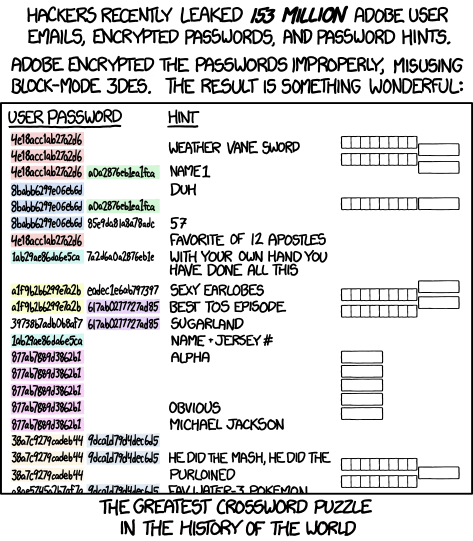
\includegraphics[width=0.75\textwidth]{figures/xkcd/xkcd_1286_encryptic.png}
    \caption[\texttt{xkcd} Encryptic]{Here we have an example of how
        \emph{not} to store passwords;
        also, see Figure~\ref{fig:xkcd_password_reuse}.
        Created by Randall Munroe on \texttt{xkcd};
        posted online at \url{https://xkcd.com/1286/}.
        }
    \label{fig:xkcd_encryptic}
\end{figure}

\begin{figure}[t]
\centering
    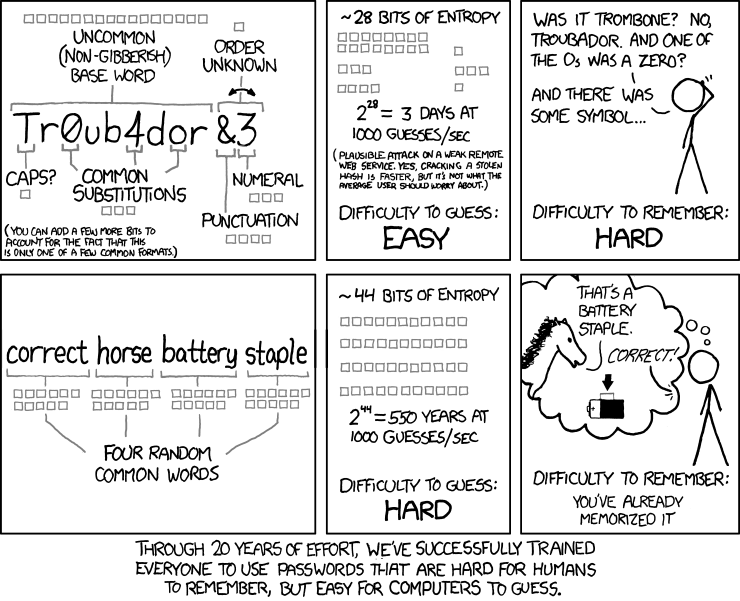
\includegraphics[width=0.75\textwidth]{figures/xkcd/xkcd_936_password_strength.png}
    \caption[\texttt{xkcd} Password Strength]{Here we learn
        about strong passwords.
        Created by Randall Munroe on \texttt{xkcd};
        posted online at \url{https://xkcd.com/936/}.
        }
    \label{fig:xkcd_password_strength}
\end{figure}

\begin{figure}[t]
\centering
    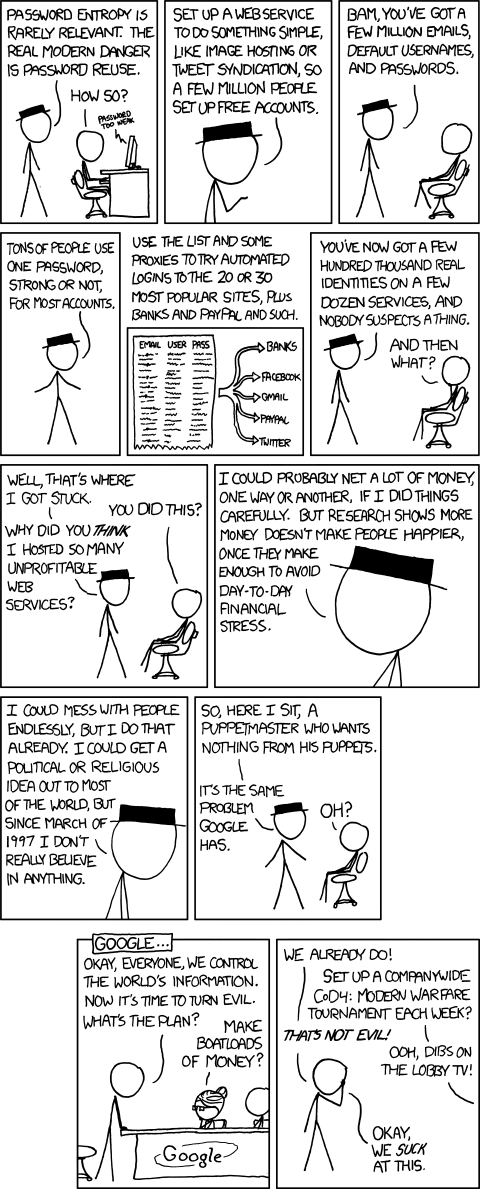
\includegraphics[width=0.5\textwidth]{figures/xkcd/xkcd_792_password_reuse.png}
    \caption[\texttt{xkcd} Password Reuse]{Here we learn
        why it is a bad idea to reuse passwords.
        Created by Randall Munroe on \texttt{xkcd};
        posted online at \url{https://xkcd.com/792/}.
        }
    \label{fig:xkcd_password_reuse}
\end{figure}


\subsection*{\Glsentrytext{salt} Length}

It is important that a \gls{salt} be long enough so that it is
impractical to form rainbow tables.
Because of this, \glspl{salt} should be at least be 128 bits (16 bytes).
Ideally, \glspl{salt} should be 256 bits (32 bytes).
Salts may be longer, but the \emph{purpose} of a \gls{salt}
is to ensure a unique output even if the same password is used multiple times.
To make the password derivation more difficult,
use a \gls{hash function} designed for password hashing and
choose the appropriate difficulty setting with iteration count
and memory requirements.



\section{Concluding Discussion of Hash Functions}

There has been a lot of information presented here on \glspl{hash function}.
From all the applications discussed, it is obvious
that \glspl{hash function} are used all over cryptography.
Also, see the discussion of geohashing in Figure~\ref{fig:xkcd_geohashing}.

\begin{figure}[t]
\centering
    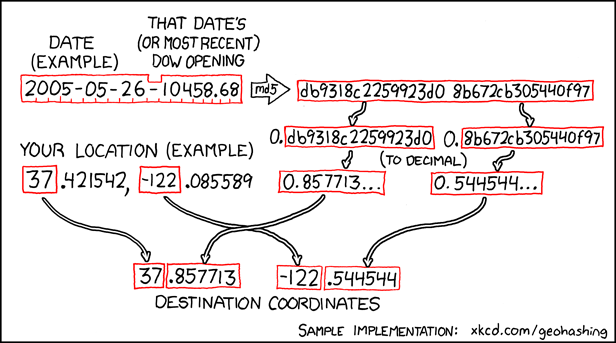
\includegraphics[width=0.75\textwidth]{figures/xkcd/xkcd_426_geohashing.png}
    \caption[\texttt{xkcd} Geohashing]{Geohashing is a
        frequently-overlooked application of \glsfirstplural{hash function}.
        Created by Randall Munroe on \texttt{xkcd};
        posted online at \url{https://xkcd.com/426/}.
        }
    \label{fig:xkcd_geohashing}
\end{figure}

